% TP Temas de Procesamiento del Lenguaje Natural — NLP Aplicado
% Grupo 6 — Universidad de Buenos Aires (FCEN, Depto. de Computación)
% Template ACL. Compilar con: latexmk -pdf main.tex
%
% Estado: estructura completa (carátula + títulos). La sección de RESULTADOS
% está redactada con datos reales; el resto de las secciones son placeholders.

\documentclass[11pt]{article}
\usepackage{acl}

\usepackage{times}
\usepackage{latexsym}
\usepackage[T1]{fontenc}
\usepackage[utf8]{inputenc}
\usepackage[spanish,es-noshorthands]{babel}
\usepackage{microtype}
\usepackage{graphicx}
\usepackage{booktabs}
\usepackage{multirow}
\usepackage{amsmath}
\usepackage{amssymb}
\usepackage{etoolbox}
\usepackage{stfloats} % permite ubicar floats de doble columna (figure*) también al pie

\graphicspath{{figuras/}}

\addto\captionsspanish{\renewcommand{\tablename}{Tabla}}
\AtBeginDocument{\patchcmd{\thebibliography}{References}{Referencias}{}{}}

\title{Evaluación humana y automática de traducción automática qom--español:\\
acuerdo entre anotadores, criterios de evaluación y métricas}

\author{
  Juan Ignacio Catania \quad Juan Cruz Mendoza \quad Camila Rodríguez \\
  Grupo 6 \\
  Universidad de Buenos Aires - FCEN \\
  2026
}

\begin{document}
\maketitle

\begin{abstract}
Abstract ...
\end{abstract}

\section{Introducción}
\label{sec:introduccion}
% TODO: Cuál es el problema, por qué es importante, qué hicieron y en qué se
% diferencia de trabajos previos. (Consigna, punto 7 — Introducción.)

\section{Metodología}
\label{sec:metodologia}

\subsection{Procedimiento de anotación}
\label{sec:metodologia-anotacion}
% TODO: Descripción de la anotación de los conjuntos A (sin guía) y C (con guía
% externa), y de la re-anotación de A con la guía propia. (Puntos 1 y 4.)
% Incluir tiempos de anotación por anotador (B y C).

\subsection{Diseño y refinamiento de la guía de anotación}
\label{sec:metodologia-guia}
% TODO: Criterios para decidir qué aspectos evaluar; dimensiones y escala;
% ejemplo anotado; dificultades y modificaciones tras probar la guía en B. (Punto 3.)

\subsection{Métricas seleccionadas}
\label{sec:metodologia-metricas}
% TODO: BLEU y BERTScore: explicación breve, justificación de la elección y
% comentarios sobre implementación. (Punto 5.)

\subsection{Data Statements}
\label{sec:metodologia-datastatements}
% TODO: Data statements de los puntos 3 y 4 (composición del equipo anotador y
% del equipo que construyó la guía externa —Grupo 5—). (Puntos 1, 2 de Referencias.)

\subsection{Detalles técnicos e implementación del IAA}
\label{sec:metodologia-tecnico}
% TODO: Decisiones de implementación; resolución de discrepancias entre
% anotadores; cómo se implementó el Alpha de Krippendorff.

\section{Resultados}
\label{sec:resultados}

Reportamos primero el acuerdo entre anotadores (IAA), luego
las métricas automáticas y, por último, su comparación con la evaluación humana.
El IAA se calculó con el Alpha de Krippendorff \citep{krippendorff2018}
(implementación de la librería \texttt{krippendorff} de Python). Las matrices de
confusión se construyeron como matrices de coincidencia agregando los tres pares
de anotadores de cada ítem. Todos los links a las anotaciones se incluyen en el
Apéndice~\ref{ap:anotaciones}.

\subsection{Acuerdo entre anotadores}
\label{sec:res-iaa}

\paragraph{Dataset A, sin criterio definido}

La evaluación libre en tres niveles se trató como ordinal
(Incorrecta${<}$Parcialmente correcta${<}$Correcta). El acuerdo fue bueno
($\alpha=0{,}79$): 10 de 15 segmentos con acuerdo unánime (67\%) y 5 con acuerdo
mayoritario (33\%), sin casos de desacuerdo total (Tabla~\ref{tab:iaa}). 

El desacuerdo casi siempre ocurre entre niveles adyacentes: en la matriz de confusión
(Fig.~\ref{fig:confusion}a) todos los pares en desacuerdo son del tipo 
Incorrecta\,/\,Parcialmente correcta o Parcialmente correcta\,/\,Correcta.

\paragraph{Dataset A, con criterio propio}

Al volver a anotar A con el criterio propio, el acuerdo fue total
($\alpha=1{,}00$ ordinal en la etiqueta global, unanimidad en los 15 segmentos). Por dimensión (escala ordinal 1--4;
Tabla~\ref{tab:dims}), el acuerdo fue alto en Fidelidad ($\alpha=0{,}96$) y
moderado en Naturalidad ($0{,}72$) y Preservación ($0{,}73$). Respecto de la
versión sin guía, $\alpha$ aumenta de $0{,}79$ a $1{,}00$. Cabe señalar que esto podría 
ser un sobreajuste, dado que la guía A fue usada para desarrollar el propio criterio.


\paragraph{Dataset B, con criterio propio}


Sobre un conjunto no empleado en el diseño de la guía, el acuerdo global fue alto
($\alpha=0{,}84$; 12/15 unánimes). Por dimensión, Fidelidad mantiene un acuerdo
elevado ($0{,}89$), mientras que Naturalidad y Preservación bajan ($0{,}31$ y
$0{,}52$). 

El bajo valor de Naturalidad coincide con un acuerdo observado alto
(13/15 unánimes) pero escasa varianza (puntajes casi siempre 3--4): al ser elevado
el acuerdo esperado por azar, $\alpha$ baja.


\paragraph{Dataset C, con criterio externo}


La guía del Grupo 5 emplea dos dimensiones (Precisión y Fluidez) en una escala continua 0--20 (Direct
Assessment, con cinco rangos), que tratamos como ordinal. El IAA se calculó sobre
los 15 segmentos anotados por los tres evaluadores. 

La Precisión muestra acuerdo alto ($\alpha=0{,}93$) y la Fluidez, moderado ($\alpha=0{,}73$). Para las
proporciones de acuerdo y la confusión redondeamos cada puntaje al rango más
cercano $\{0,5,10,15,20\}$: en Precisión, 8/15 unánimes y 7/15 mayoritarios. 
En Fluidez, 9/15 unánimes, 4 mayoritarios y 2 en desacuerdo total. 

\begin{table}[t]
\centering
\small
\begin{tabular}{lccccc}
\toprule
Conjunto (global) & Escala & $\alpha$ & 3/3 & 2/3 & 0/3 \\
\midrule
A sin guía       & ordinal & 0{,}79 & 67\% & 33\% & 0\% \\
A con guía       & ordinal & 1{,}00 & 100\% & 0\% & 0\% \\
B con guía       & ordinal & 0{,}84 & 80\% & 20\% & 0\% \\
C -- Precisión   & ordinal & 0{,}93 & 53\% & 47\% & 0\% \\
C -- Fluidez     & ordinal & 0{,}73 & 60\% & 27\% & 13\% \\
\bottomrule
\end{tabular}
\caption{IAA (Alpha de Krippendorff) y proporciones de acuerdo con $N=15$ en todos los casos. En C,
$\alpha$ se computa sobre los puntajes crudos 0--20 y las proporciones sobre los
valores redondeados a los rangos.}
\label{tab:iaa}
\end{table}

\begin{table}[t]
\centering
\small
\begin{tabular}{lcccc}
\toprule
 & \multicolumn{2}{c}{A (con guía)} & \multicolumn{2}{c}{B} \\
\cmidrule(lr){2-3}\cmidrule(lr){4-5}
Dimensión & $\alpha$ & 3/3 & $\alpha$ & 3/3 \\
\midrule
Fidelidad    & 0{,}96 & 87\% & 0{,}89 & 67\% \\
Naturalidad  & 0{,}72 & 60\% & 0{,}31 & 87\% \\
Preservación & 0{,}73 & 73\% & 0{,}52 & 47\% \\
\bottomrule
\end{tabular}
\caption{IAA por dimensión de la guía propia (escala ordinal 1--4, $N=15$).}
\label{tab:dims}
\end{table}

\begin{figure*}[!t]
\centering
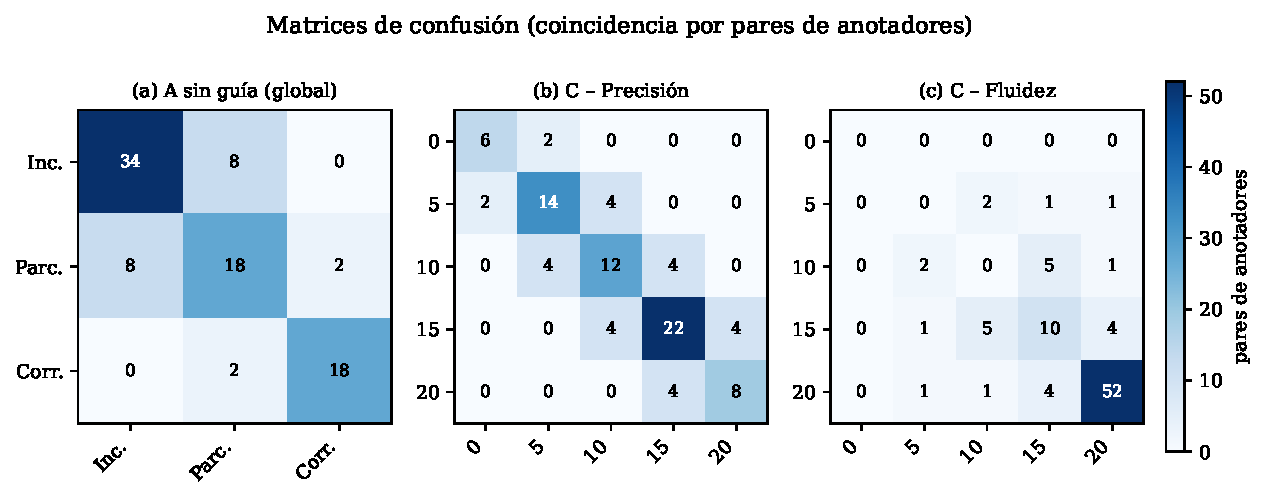
\includegraphics[width=0.92\textwidth]{confusion.pdf}
\caption{Matrices de confusión por pares de anotadores. Cada ítem aporta sus 3
pares, contabilizados de forma simétrica (un par que coincide suma 2 en la
diagonal). (a) Conjunto A sin guía, etiqueta global; (b) y (c) Precisión y
Fluidez del conjunto C, redondeadas a los rangos 0--20.}
\label{fig:confusion}
\end{figure*}

\subsection{Métricas automáticas}
\label{sec:res-metricas}

Calculamos BLEU con sacreBLEU \citep{post2018call,papineni2002bleu} y BERTScore
\citep{zhang2020bertscore}, comparando la salida automática contra la referencia en
español sobre los 120 segmentos únicos del conjunto C (15 compartidos más 35 por
anotador). BLEU se computa a nivel de corpus (tokenización \texttt{13a}) y,
para la correlación, a nivel de oración (con smoothing exponencial);
BERTScore se reporta como media de los puntajes por oración (no posee variante de
corpus) y se computó con el modelo multilingüe \texttt{bert-base-multilingual-cased}
(\texttt{lang=es}), con reescalado oficial respecto de la línea base. La
Tabla~\ref{tab:metricas} indica el nivel de agregación de cada métrica.

\begin{table}[t]
\centering
\small
\begin{tabular}{llc}
\toprule
Métrica & Nivel & Valor \\
\midrule
BLEU            & corpus            & 28{,}8 \\
BLEU            & oración (media)   & 45{,}3 \\
BLEU            & oración (mediana) & 37{,}7 \\
BERTScore F1        & oración (media) & 0{,}656 \\
BERTScore Precisión & oración (media) & 0{,}681 \\
BERTScore Recall    & oración (media) & 0{,}634 \\
\bottomrule
\end{tabular}
\caption{Métricas automáticas sobre el conjunto C ($N=120$), con el nivel de
agregación de cada una. sacreBLEU 2.6.0 (\texttt{13a}; smoothing exp a nivel
de oración); BERTScore con el modelo multilingüe (\texttt{bert-base-multilingual-cased})
y reescalado oficial respecto de la línea base \citep{zhang2020bertscore}.}
\label{tab:metricas}
\end{table}

Sin reescalado, los valores absolutos de BERTScore no son directamente
interpretables: por la similitud de base entre oraciones en español, incluso pares
no relacionados reciben puntajes altos. El reescalado oficial respecto de la línea
base \citep{zhang2020bertscore} corrige esto ubicando esos pares cerca de 0, y deja
el F1 en $0{,}656$. 

El valor de BLEU debe leerse en el contexto de bajos
recursos: como referencia de literatura, en el shared task AmericasNLP 2025
\citep{degibert2025findings} el mejor sistema de traducción hacia el español
promedia BLEU $\approx 7{,}2$ sobre 13 lenguas indígenas (allí la métrica principal
es chrF++). El qom no integra ese conjunto y los segmentos de C son breves, por lo que la comparación es 
solo orientativa: el BLEU de $28{,}8$
refleja en buena medida esa diferencia de tarea (lengua, dirección y longitud de
los segmentos) más que necesariamente un sistema superior.

\subsection{Comparación humana vs.\ automática}
\label{sec:res-comparacion}

Para cada segmento de C tomamos como ground truth el promedio de los anotadores
(tres en los segmentos compartidos, uno en el resto) y lo correlacionamos con cada
métrica mediante el coeficiente de Pearson ($r$). Ambas métricas se correlacionan
de forma significativa con el juicio humano y, en todos los casos, más con
Precisión que con Fluidez, lo cual es esperable dado que miden similitud con la
referencia (Tabla~\ref{tab:corr}, Fig.~\ref{fig:scatter}). 

BERTScore supera a BLEU frente a las tres variables humanas. El patrón se mantiene al restringir el
análisis a los 15 segmentos compartidos (promediados sobre tres anotadores):
BERTScore--Precisión $r=0{,}82$ y BLEU--Precisión $r=0{,}61$, mientras que la
correlación con Fluidez no resulta significativa.

\begin{table}[t]
\centering
\small
\begin{tabular}{lccc}
\toprule
Métrica & Precisión & Fluidez & Global \\
\midrule
BLEU (oración)        & 0{,}69 & 0{,}31 & 0{,}62 \\
BERTScore F1 (oración) & 0{,}78 & 0{,}45 & 0{,}74 \\
\bottomrule
\end{tabular}
\caption{Correlación de Pearson ($r$) entre cada métrica (a nivel de oración) y el
juicio humano ($N=120$).}
\label{tab:corr}
\end{table}

\begin{figure*}[!t]
\centering
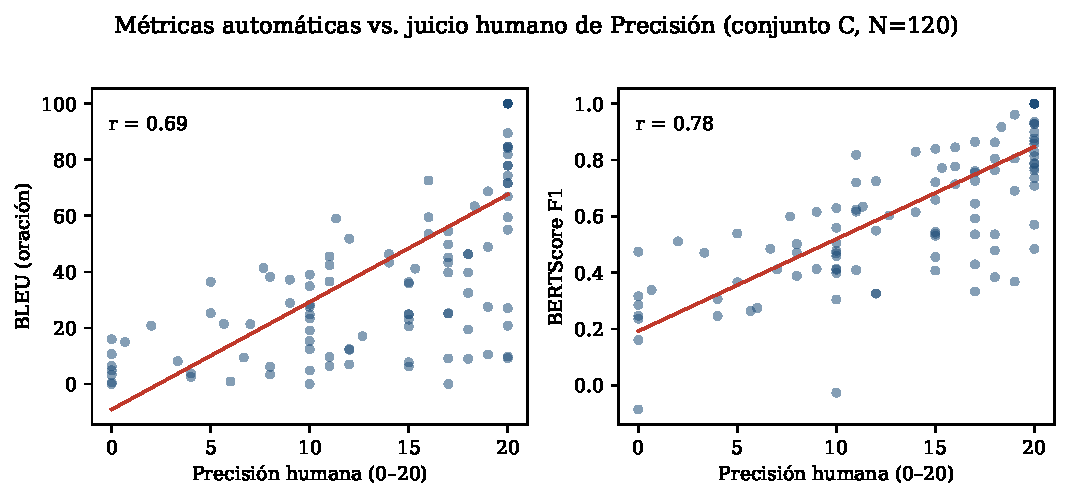
\includegraphics[width=0.78\textwidth]{scatter.pdf}
\caption{Métricas automáticas frente al juicio humano de Precisión (conjunto C,
$N=120$). La recta es el ajuste lineal y $r$ es el coeficiente de Pearson.}
\label{fig:scatter}
\end{figure*}



\section{Discusión}
\label{sec:discusion}
% TODO: Principales dificultades; limitaciones de las métricas; recomendaciones
% para futuras evaluaciones. Discutir que el conjunto A se usó al elaborar y
% refinar la guía: implicancias para interpretar el cambio de IAA entre la
% versión sin guía y con guía; ¿el acuerdo sobre A refleja la calidad general de
% la guía? (Punto 7 — Discusión; preguntas del punto 6.)

\section{Conclusiones}
\label{sec:conclusiones}
% TODO: Conclusiones del trabajo.


\bibliography{referencias}

\appendix
\section{Anotaciones (enlaces)}
\label{ap:anotaciones}

Las planillas con las anotaciones completas están disponibles en los siguientes
enlaces:
\begin{itemize}
  \item \textbf{Conjunto A} (sin criterio):
    \href{https://docs.google.com/spreadsheets/d/1sNausxIyKAkPQqZLzBhwwcWVJZw6RVvCREiOsXESHJA/edit?gid=197319219\#gid=197319219}{enlace}.
  \item \textbf{Conjunto A} (con criterio propio):
    \href{https://docs.google.com/spreadsheets/d/10D6LHwRfZ-UI1jfoNbYCG6vAj-GPCtuhSARlbtt4Iwo/edit?gid=239714396\#gid=239714396}{enlace}.
  \item \textbf{Conjunto B} (criterio propio):
    \href{https://docs.google.com/spreadsheets/d/1RuGaMAdIc9IuWvecUwBUUF0Egr-905_fVvoCKso3fWE/edit?gid=741315237\#gid=741315237}{enlace}.
  \item \textbf{Conjunto C} (criterio externo):
    \href{https://docs.google.com/spreadsheets/d/1l7rSK5nfPkUuYa_YYcUt0vB9ZpxL_bLsJTQWG82fqlQ/edit?gid=1957930832\#gid=1957930832}{enlace}.
\end{itemize}

\section{Tablas y material complementario}
\label{ap:complementario}
% TODO: tablas extendidas / material adicional si corresponde.


\end{document}
